%%%%%%%%%%%%%%%%%%%%%%%%%%%%%%%%%%%%%%%%%
% Make sure to set your name, legi number and url to the right git branch.

\newcommand{\hmwkAuthorName}{Zhejun Zhang} % Your name
\newcommand{\hmwkAuthorLegi}{16-930-612} % Your name
\newcommand{\hmwkGitBranch}{https://gitlab.vis.ethz.ch/vwegmayr/slt-coding-exercises/tree/16-930-612/1\_locally\_linear\_embedding} % Your name
%
%%%%%%%%%%%%%%%%%%%%%%%%%%%%%%%%%%%%%%%%%

%----------------------------------------------------------------------------------------
%	PACKAGES AND OTHER DOCUMENT CONFIGURATIONS
%	Skip this
%----------------------------------------------------------------------------------------

\documentclass{article}

\usepackage{amsfonts}
\usepackage[T1]{fontenc}
\usepackage{fancyhdr} % Required for custom headers
\usepackage{lastpage} % Required to determine the last page for the footer
\usepackage{extramarks} % Required for headers and footers
\usepackage{graphicx} % Required to insert images
\usepackage{lipsum} % Used for inserting dummy 'Lorem ipsum' text into the template

% Margins
\topmargin=-0.45in
\evensidemargin=0in
\oddsidemargin=0in
\textwidth=6.5in
\textheight=9.0in
\headsep=0.25in 

\linespread{1.1} % Line spacing

% Set up the header and footer
\pagestyle{fancy}
\lhead{\hmwkAuthorName} % Top left header
\chead{\hmwkClass\ \hmwkTitle} % Top center header
\rhead{\firstxmark} % Top right header
\lfoot{\lastxmark} % Bottom left footer
\cfoot{} % Bottom center footer
\rfoot{Page\ \thepage\ of\ \pageref{LastPage}} % Bottom right footer
\renewcommand\headrulewidth{0.4pt} % Size of the header rule
\renewcommand\footrulewidth{0.4pt} % Size of the footer rule

\setlength\parindent{0pt} % Removes all indentation from paragraphs

%----------------------------------------------------------------------------------------
%	DOCUMENT STRUCTURE COMMANDS
%	Skip this
%----------------------------------------------------------------------------------------

% Header and footer for when a page split occurs within a problem environment
\newcommand{\enterProblemHeader}[1]{
\nobreak\extramarks{#1}{#1 continued on next page\ldots}\nobreak
\nobreak\extramarks{#1 (continued)}{#1 continued on next page\ldots}\nobreak
}

% Header and footer for when a page split occurs between problem environments
\newcommand{\exitProblemHeader}[1]{
\nobreak\extramarks{#1 (continued)}{#1 continued on next page\ldots}\nobreak
\nobreak\extramarks{#1}{}\nobreak
}

\setcounter{secnumdepth}{0} % Removes default section numbers
\newcounter{homeworkProblemCounter} % Creates a counter to keep track of the number of problems

\newcommand{\homeworkProblemName}{}
\newenvironment{homeworkProblem}[1][Problem \arabic{homeworkProblemCounter}]{ % Makes a new environment called homeworkProblem which takes 1 argument (custom name) but the default is "Problem #"
\stepcounter{homeworkProblemCounter} % Increase counter for number of problems
\renewcommand{\homeworkProblemName}{#1} % Assign \homeworkProblemName the name of the problem
\section{\homeworkProblemName} % Make a section in the document with the custom problem count
\enterProblemHeader{\homeworkProblemName} % Header and footer within the environment
}{
\exitProblemHeader{\homeworkProblemName} % Header and footer after the environment
}

\newcommand{\problemAnswer}[1]{ % Defines the problem answer command with the content as the only argument
\noindent\framebox[\columnwidth][c]{\begin{minipage}{0.98\columnwidth}#1\end{minipage}} % Makes the box around the problem answer and puts the content inside
}

\newcommand{\homeworkSectionName}{}
\newenvironment{homeworkSection}[1]{ % New environment for sections within homework problems, takes 1 argument - the name of the section
\renewcommand{\homeworkSectionName}{#1} % Assign \homeworkSectionName to the name of the section from the environment argument
\subsection{\homeworkSectionName} % Make a subsection with the custom name of the subsection
\enterProblemHeader{\homeworkProblemName\ [\homeworkSectionName]} % Header and footer within the environment
}{
\enterProblemHeader{\homeworkProblemName} % Header and footer after the environment
}
   
%----------------------------------------------------------------------------------------
%	NAME AND CLASS SECTION
%	Skip this
%----------------------------------------------------------------------------------------

\newcommand{\hmwkTitle}{Locally Linear Embedding} % Assignment title
\newcommand{\hmwkDueDate}{Monday,\ March\ 6th,\ 2017} % Due date
\newcommand{\hmwkClass}{SLT coding exercise\ \#1} % Course/class
\newcommand{\hmwkClassTime}{Mo 16:15} % Class/lecture time
\newcommand{\hmwkClassInstructor}{} % Teacher/lecturer

%----------------------------------------------------------------------------------------
%	TITLE PAGE
%	Skip this
%----------------------------------------------------------------------------------------

\title{
\vspace{2in}
\textmd{\small{\hmwkClass}}\\
\textmd{\textbf{\hmwkTitle}}\\
\small{https://gitlab.vis.ethz.ch/vwegmayr/slt-coding-exercises}\\
\normalsize\vspace{0.1in}\small{Due\ on\ \hmwkDueDate}
%\vspace{0.1in}\large{\textit{\hmwkClassInstructor\ \hmwkClassTime}}
\vspace{3in}
}

\author{
\hmwkAuthorName\\
\hmwkAuthorLegi
}

\date{ } % Insert date here if you want it to appear below your name

\begin{document}

\maketitle

%----------------------------------------------------------------------------------------
%	TABLE OF CONTENTS
%	Skip this
%----------------------------------------------------------------------------------------

%\setcounter{tocdepth}{1} % Uncomment this line if you don't want subsections listed in the ToC

\newpage
\tableofcontents
\newpage

%----------------------------------------------------------------------------------------
%	SECTIONS
%	Now you are in the right hood
%----------------------------------------------------------------------------------------

\begin{homeworkProblem}[The Model]
The model section is intended to allow you to recapitulate the essential ingredients used in \hmwkTitle. Write down the \textit{necessary} equations to specify \hmwkTitle\ and and shortly explain the variables that are involved. This section should only introduce the equations, their solution should be outlined in the implementation section.\newline
Hard limit: One page
\vspace{10pt}

\problemAnswer{ % Answer
LLE is used to reduce the dimensionality of data set. Given a set of $N$ points $\mathbf{x}_i \in \mathbb{R}^D, i=1,..,N$, LLE will find the corresponding points $\mathbf{y}_i \in \mathbb{R}^d, i=1,..,N, d\ll D$ in a lower dimensional space. Basically, LLE contains the following steps.\\
\\
(1) Find matrix $\mathbf{W}$ such that it satisfies
\begin{equation}
\sum_j w_{ij}=1
\end{equation}
and minimizes
\begin{equation} \label{error_x}
\varepsilon(\mathbf{W})=\sum_i \left\| \mathbf{x}_i -\sum_{j\in \mathcal{N}(\mathbf{x}_i)} w_{ij}\mathbf{x}_j\right\|^2,
\end{equation}
where $\mathcal{N}(\mathbf{x}_i)$ is the index set for the neighboring points of point $\mathbf{x}_i$.
\\

(2) Find $\mathbf{y}_i\in \mathbb{R}^d, i=1,..,N$ such that they satisfy
\begin{equation}
\sum_i \mathbf{y}_i=\mathbf{0}
\end{equation}
\begin{equation}
\sum_i\mathbf{y}_i\mathbf{y}_i^\top=\mathbb{I}
\end{equation}
and minimize
\begin{equation}\label{error_y}
\varepsilon(\mathbf{\mathbf{y}_1,...,\mathbf{y}_N})=\sum_i \left\| \mathbf{y}_i -\sum_{j\in \mathcal{N}(\mathbf{y}_i)} w_{ij}\mathbf{y}_j\right\|^2,
\end{equation}
where $w_{ij}$ are entries of matrix $\mathbf{W}$ founded in step (1). In principle, the neighborhood sets $\mathcal{N}(\mathbf{x}_i)$ and $\mathcal{N}(\mathbf{y}_i)$ are the same.






}
\end{homeworkProblem}
\clearpage

%----------------------------------------------------------------------------------------
\begin{homeworkProblem}[The Questions]
This is the core section of your report, which contains the tasks for this exercise and your respective solutions. Make sure you present your results in an illustrative way by making use of graphics, plots, tables, etc. so that a reader can understand the results with a single glance. Check that your graphics have enough resolution or are vector graphics. Consider the use of GIFs when appropriate.\newline
Hard limit: Two pages

\begin{homeworkSection}{(a) Get the data}
For this exercise we will work with the MNIST data set. In order to learn more about it and download it, go to http://yann.lecun.com/exdb/mnist/.
\end{homeworkSection}

\begin{homeworkSection}{(b) Locally linear embedding}
Implement the LLE algorithm and apply it to the MNIST data set. Provide descriptive visualizations for 2D \& 3D embedding spaces. Is it possible to see clusters?
\end{homeworkSection}

\begin{homeworkSection}{(c) Cluster structure}
Investigate the cluster structure of the data. Can you observe block structures in the $M$ matrix (use matrix plots)? Also plot the singular values of $M$. Do you notice something?
Can you think of ways to determine the optimal embedding dimension?
\end{homeworkSection}

\begin{homeworkSection}{(d) Nearest Neighbors}
Investigate the influence of the choice of how many nearest neighbors you take into account. Additionally, try different metrics to find the nearest neighbors (we are dealing with images!).
\end{homeworkSection}

\begin{homeworkSection}{(e) Linear manifold interpolation}
Assume you pick some point in the embedding space. How can you map it back to the original (high dimensional) space? Investigate how well this works for points within and outside the manifold (does it depend on the dimensionality of the embedding space?) Try things like linearly interpolating between two embedding vectors and plot the sequence of images along that line. What happens if you do that in the original space?
\end{homeworkSection}

\vspace{10pt}
\problemAnswer{ % Answer
(b) The left figure demonstrates 2D embedding space. The right figure shows 3D embedding space. The data sets include 1000 images. In both figure the 1-norm and five neighborhoods are used. Clusters can be distinguished easily in both 2D and 3D embedding space. Clusters that cannot be distinguished in 2D embedding space, like 4 and 7, are possible to be separated in a 3D embedding space along the third additional direction.

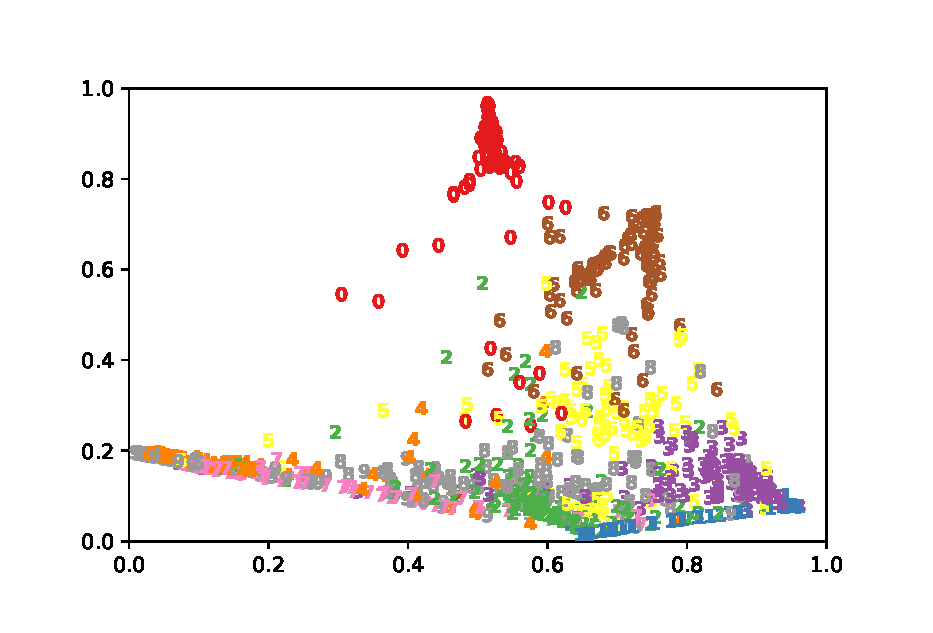
\includegraphics[scale=0.5]{norm1n5.eps}
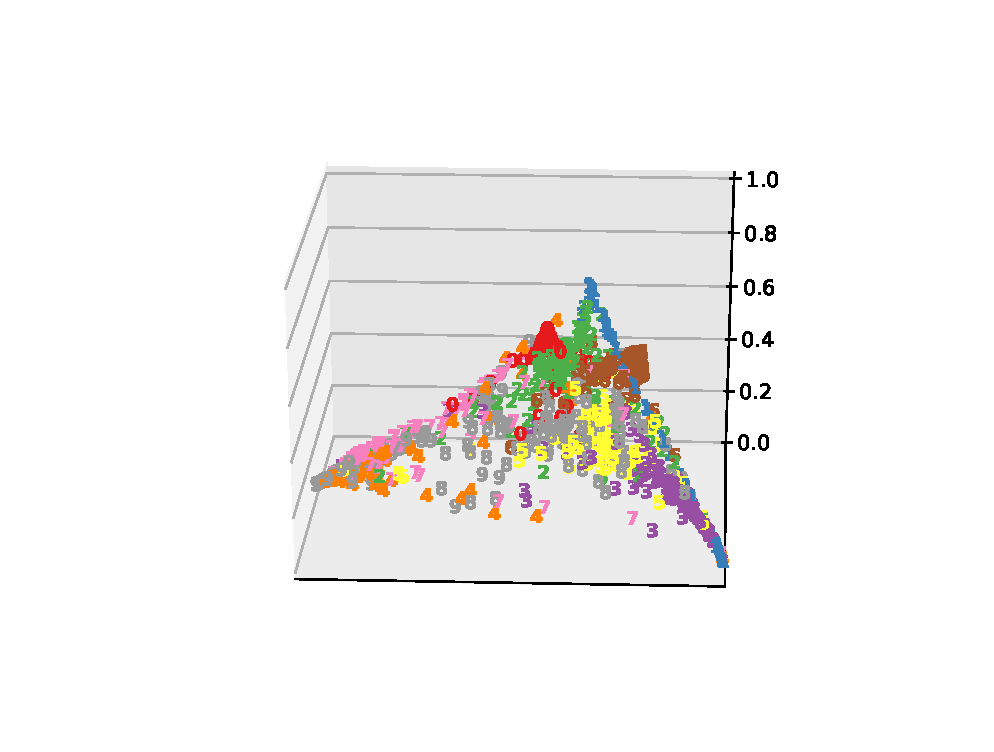
\includegraphics[scale=0.5]{3dnorm1n5.eps}\\

(c) Matrix $M$ has a diagonal structure and is very sparse. We cannot observe obvious block structures in the $M$ matrix. Since $M$ is a symmetric, positive definite matrix, its singular values are identical to its eigenvalues. The eigenvalues of $M$ are plotted on the right figure. We notice after 800, the eigenvalue begins to increase dramatically. But most eigenvalues are small and close to zero. Greater eigenvalues lead to larger reconstruction errors and are thus less informative. This implies us to choose the optimal embedding dimension $d$ such the $d$th greatest eigenvalue is still close to zero. Therefore the optimal embedding dimension should be smaller than 600.
\\
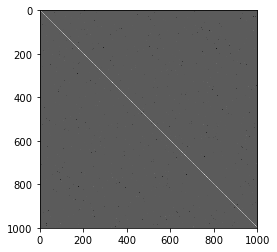
\includegraphics[ width=.35\textwidth]{M.png}
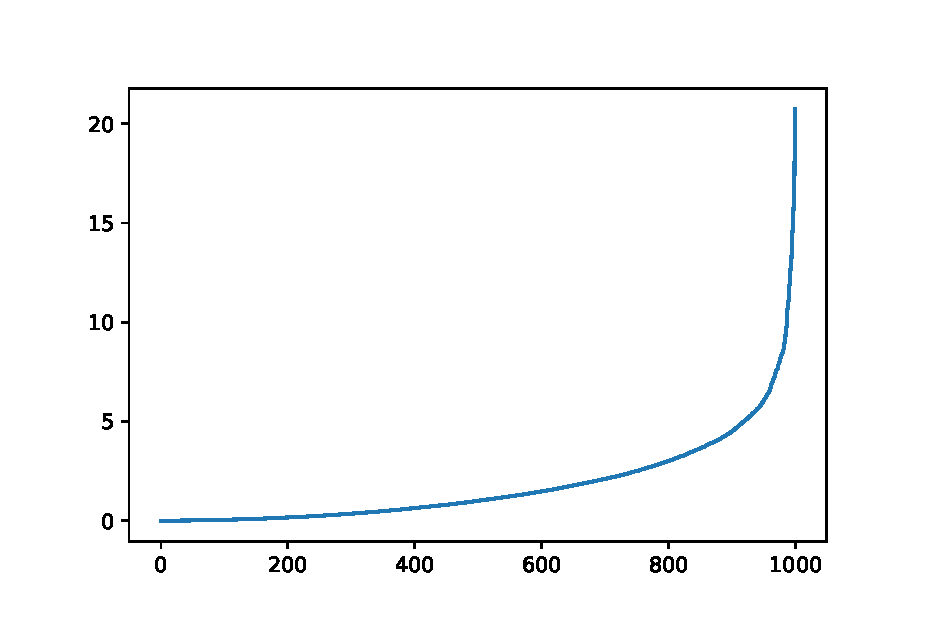
\includegraphics[width=.5\textwidth]{ev.eps}\\

(d) The following two figures show the 2D embedding space if we use 30 neighbors (left) and 50 neighbors (right). The used metric is still 1-norm. Clusters can still be distinguished but more of them overlapped with each other. It seems for a lower dimensional embedding space, considering more neighbors in the computation doesn't necessarily make it easier to separate clusters. This is mostly likely because the data set we use is rather small (1000 images). For a good clustering effect, we want neighbors of a image have the same label as that image.


}

\problemAnswer{ % Answer

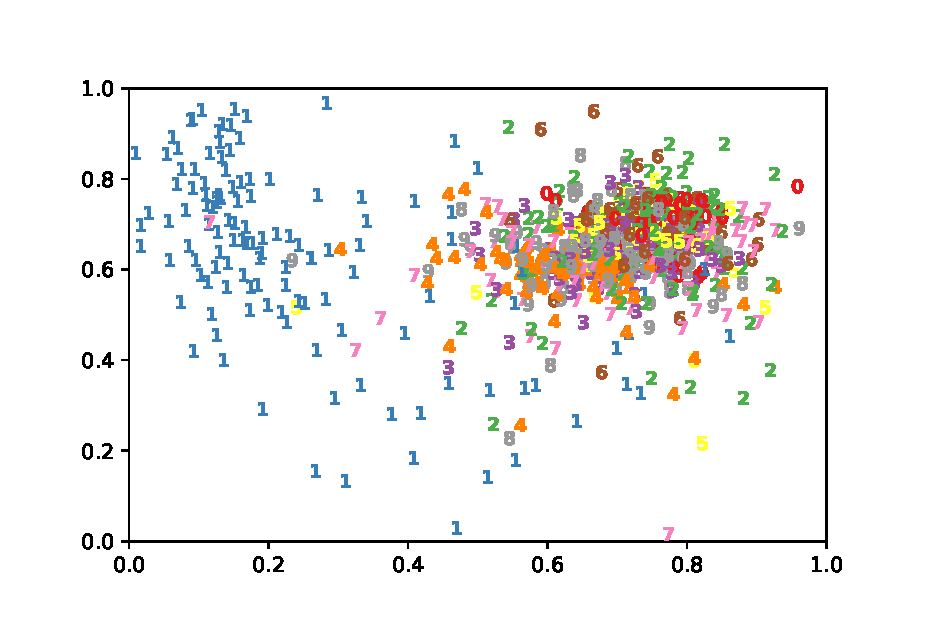
\includegraphics[width=.5\textwidth]{norm1n30.eps}
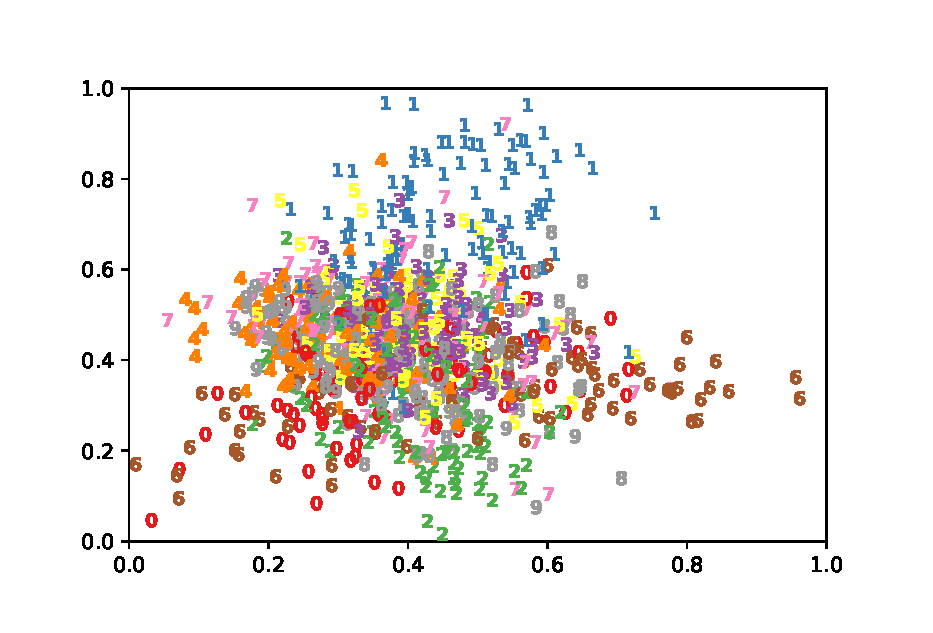
\includegraphics[width=.5\textwidth]{norm1n50.eps}

Before we used 1-norm. Now we try 2-norm, the Euclidean norm. The results are shown in the following figures. Left with 5 neighbors and right with 30 neighbors. It seems for MNIST dataset, 1-norm gives rise to more distinguishable clusters. But the results of 2-norm are not meaningless. Clusters still exist.

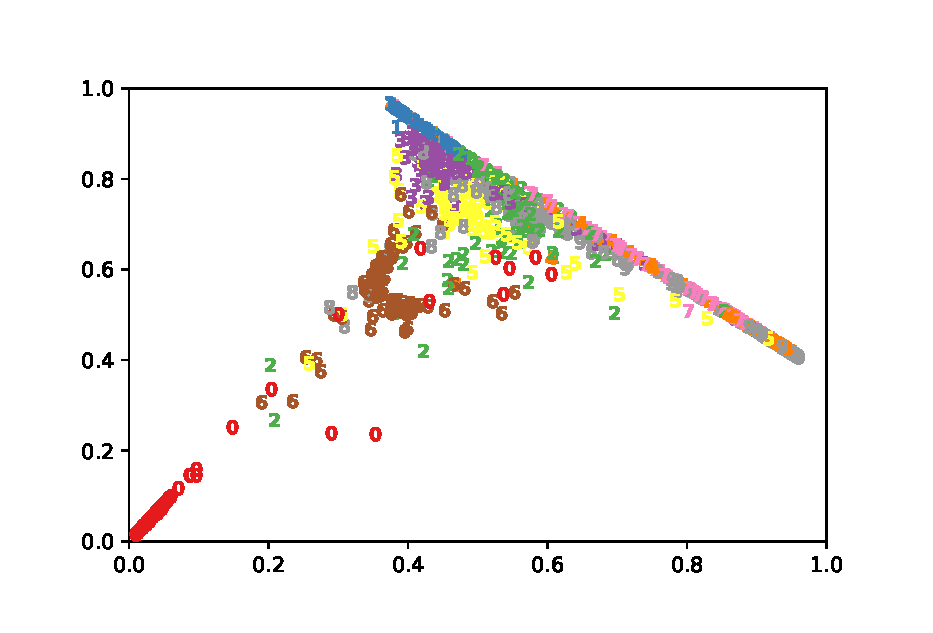
\includegraphics[width=.5\textwidth]{norm2n5.eps}
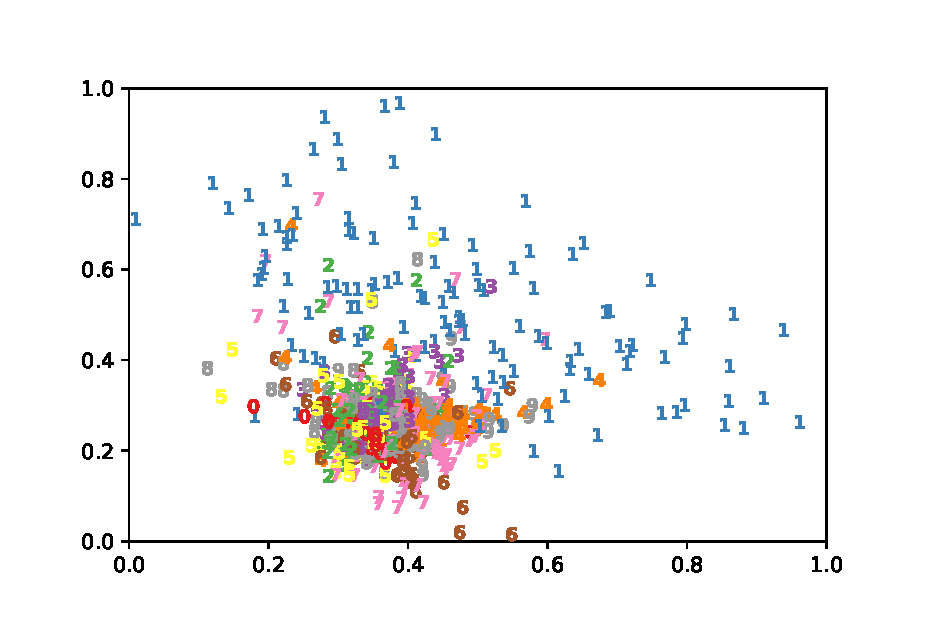
\includegraphics[width=.5\textwidth]{norm2n30.eps}

(e) 
The inverse mapping of a point $\mathbf{y}$ in the embedding space can be found by first finding neighbors of $\mathbf{y}$ in the embedding space. Then solve the optimization as defined in equation \ref{error_x} but replacing $\mathbf{x}_i$ with $\mathbf{y}$ and $\mathbf{x}_j$ with neighbors of $\mathbf{y}$. The outcome of this optimization problem is a $n\times1$ weight vector $\mathbf{w}$. Then the inverse mapping can be found by computing the weighted sum of all inverse mappings of $\mathbf{y}$'s neighbors using $\mathbf{w}$ as weight.

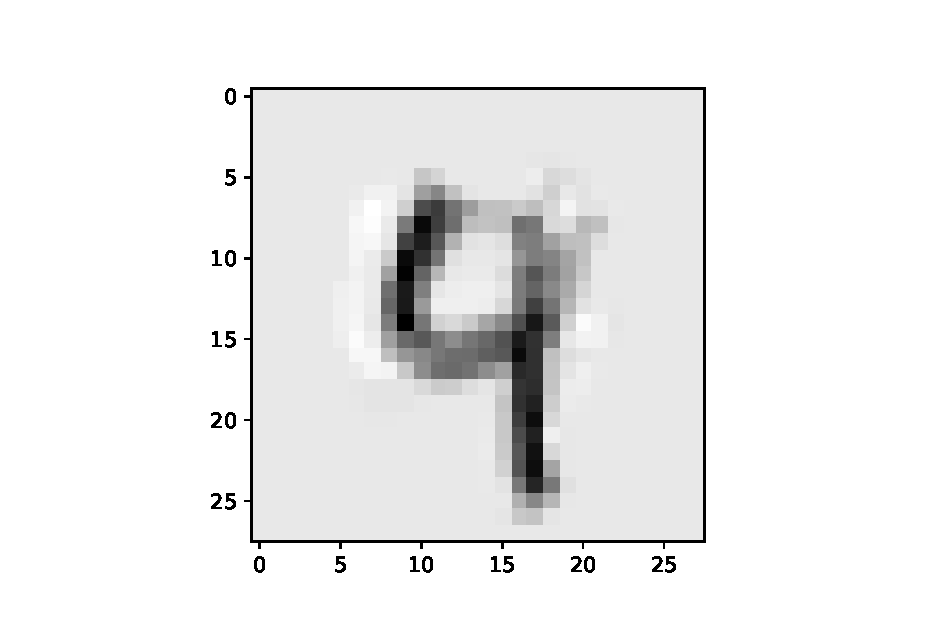
\includegraphics[width=.16\textwidth]{p0.eps}
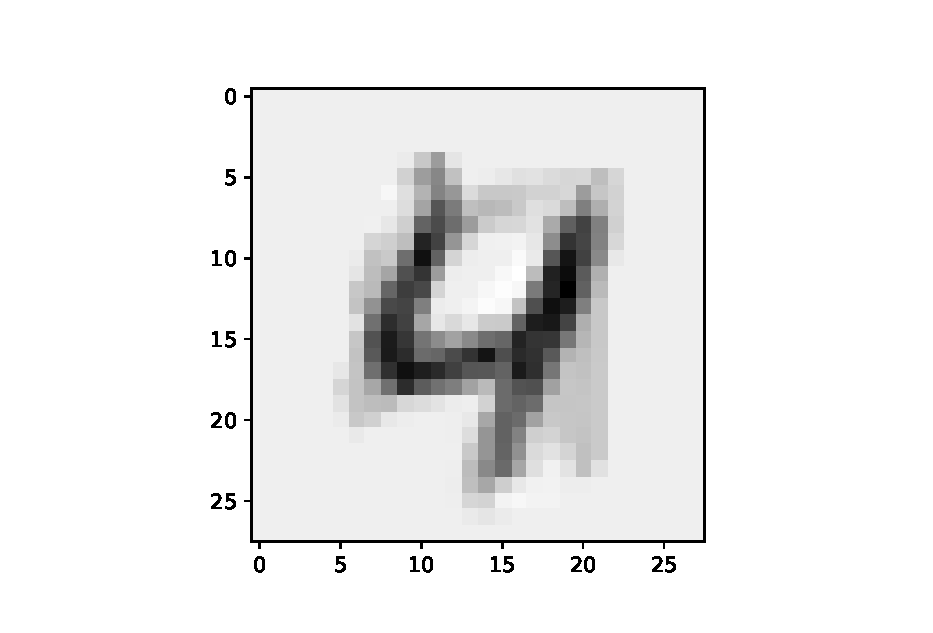
\includegraphics[width=.16\textwidth]{p2.eps}
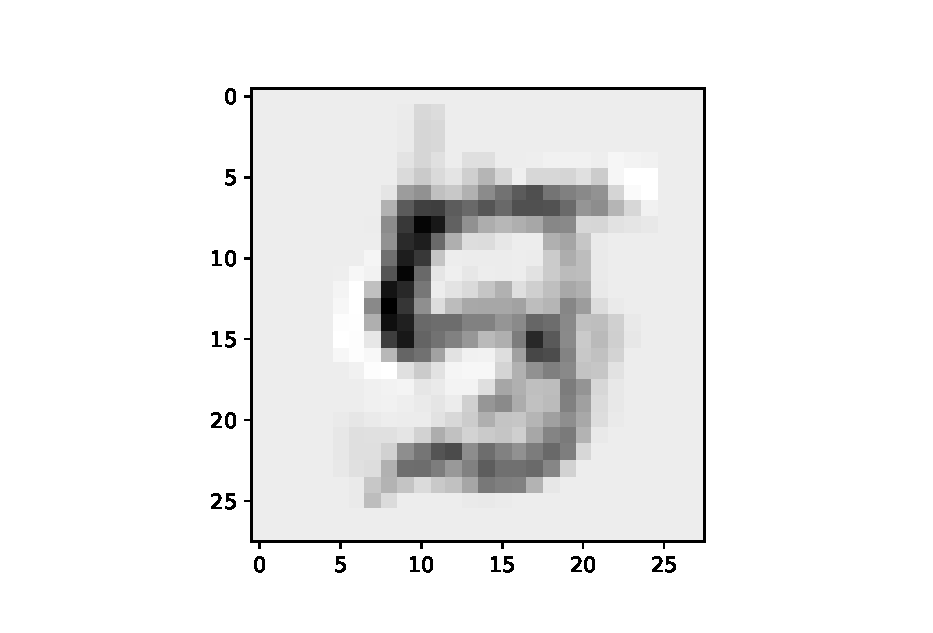
\includegraphics[width=.16\textwidth]{p4.eps}
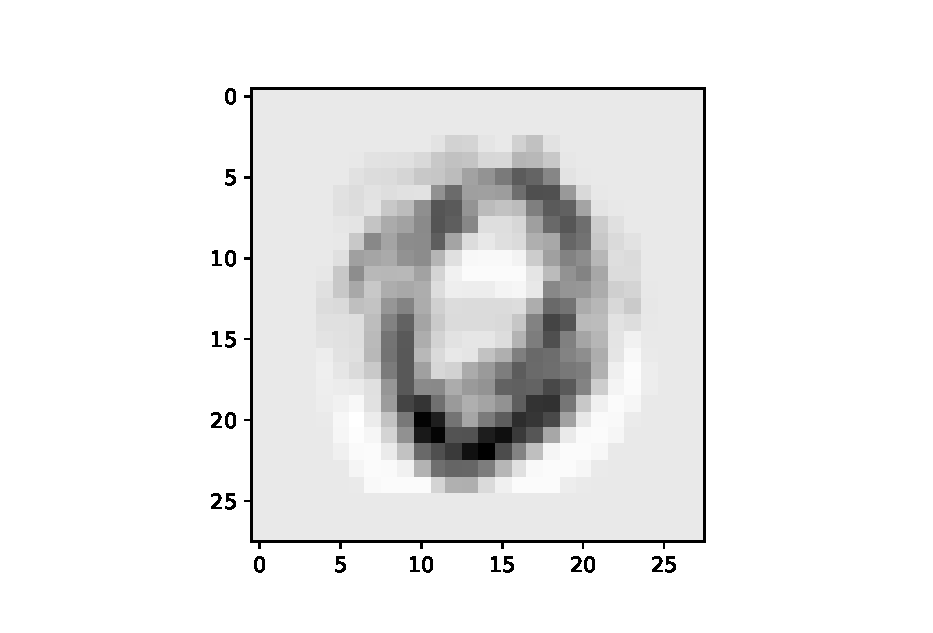
\includegraphics[width=.16\textwidth]{p6.eps}
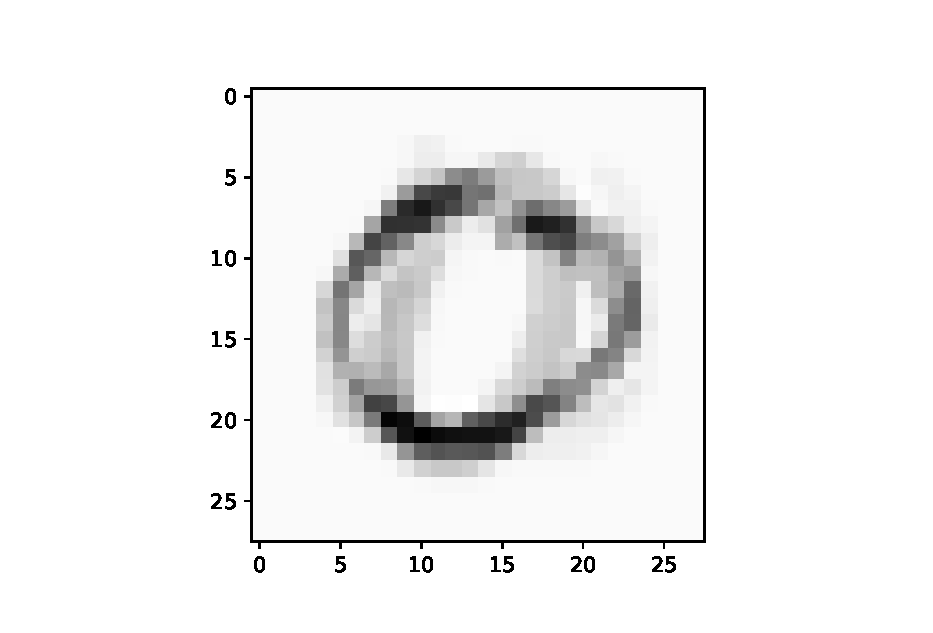
\includegraphics[width=.16\textwidth]{p8.eps}
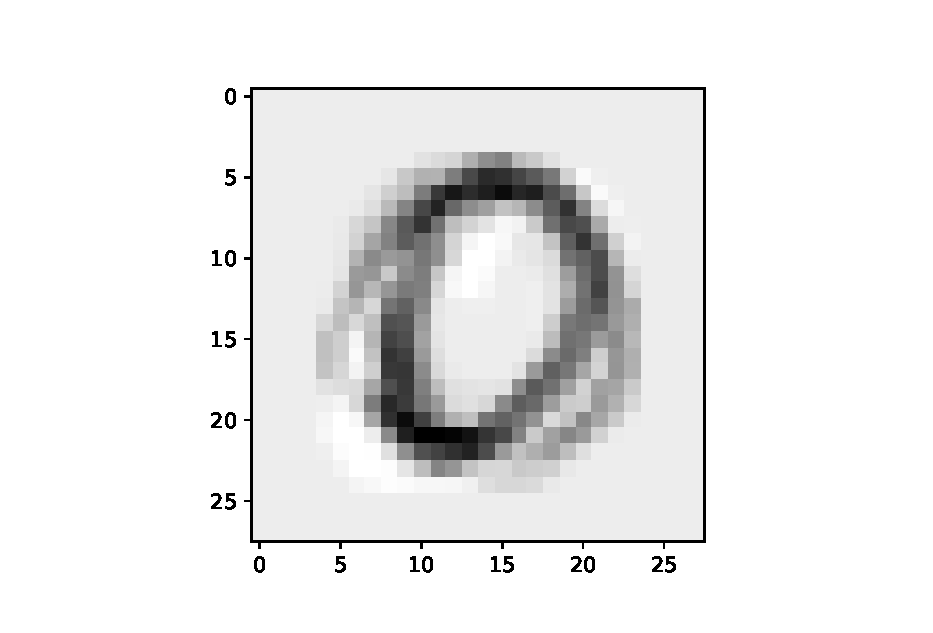
\includegraphics[width=.16\textwidth]{p10.eps} 

These figures show the reconstructed images along the linear interpolation between two points in the embedding space. In above figures, the coefficients for the linear interpolation between number four and number zero are 0, 0.2, 0.4, 0.6, 0.8 and 1 from left to right. We notice if stay closed to the manifold, the reconstructed image is reasonable. But for points outside the manifold (for example both images in the middle), the reconstructed image is rather noisy. This is because the clusters are not well separated. There are many other attractors between both given embedding vectors (here 4 and 0).

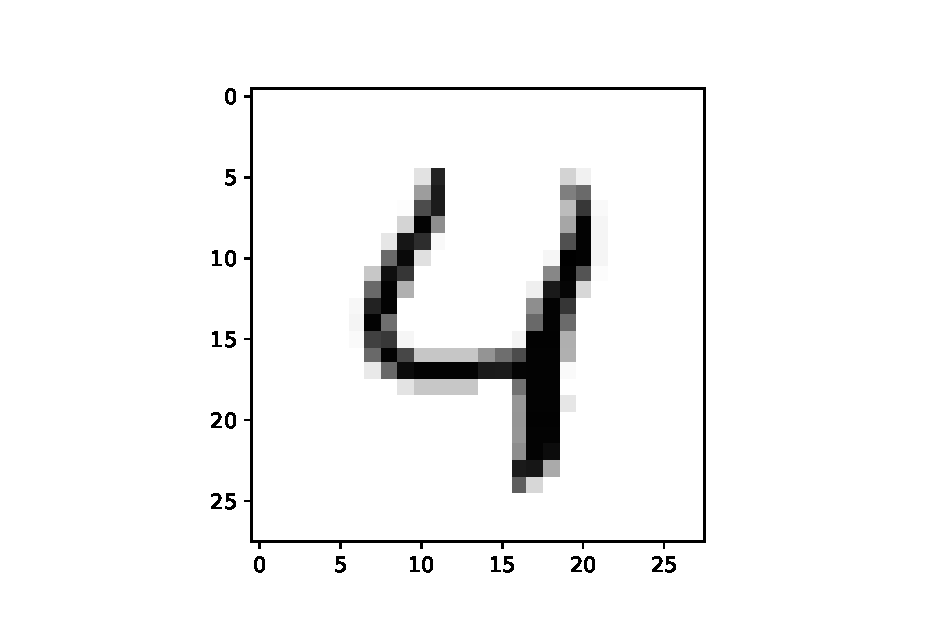
\includegraphics[width=.16\textwidth]{x0.eps}
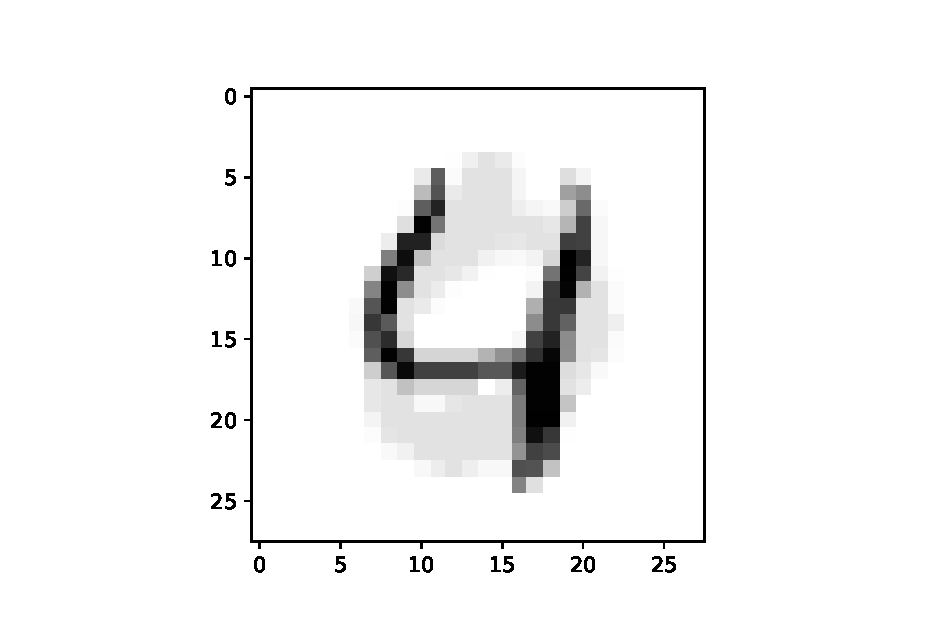
\includegraphics[width=.16\textwidth]{x2.eps}
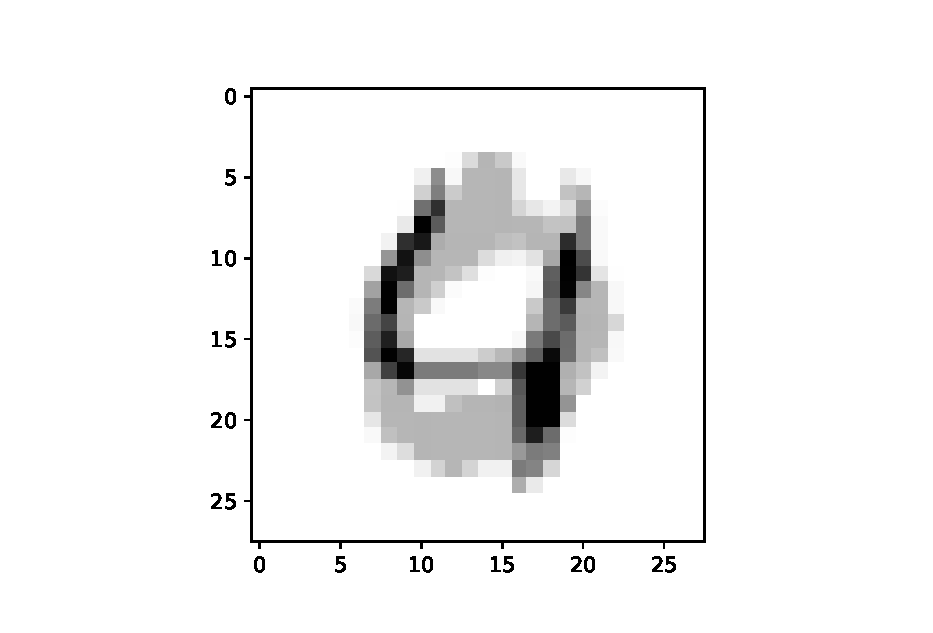
\includegraphics[width=.16\textwidth]{x4.eps}
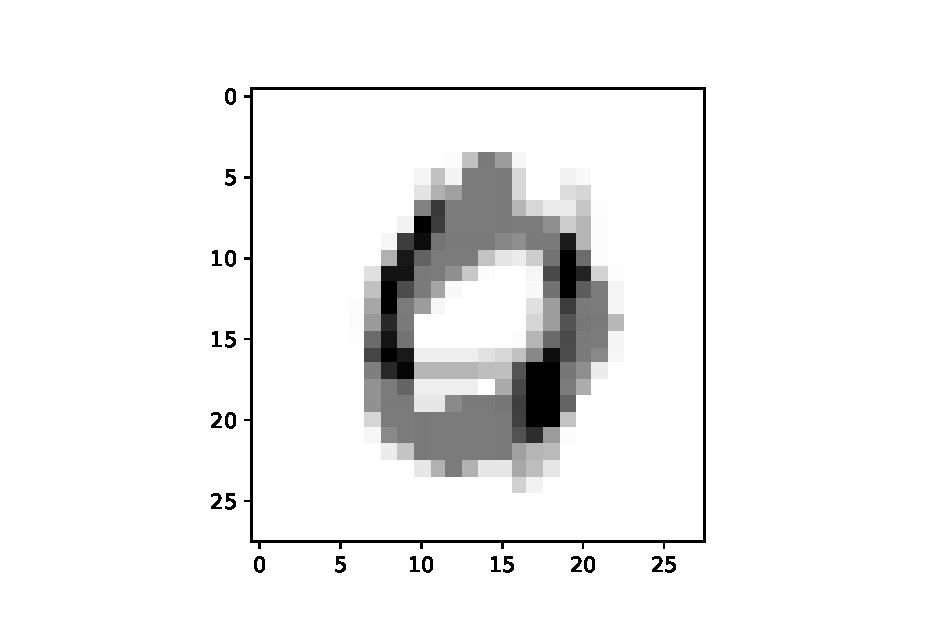
\includegraphics[width=.16\textwidth]{x6.eps}
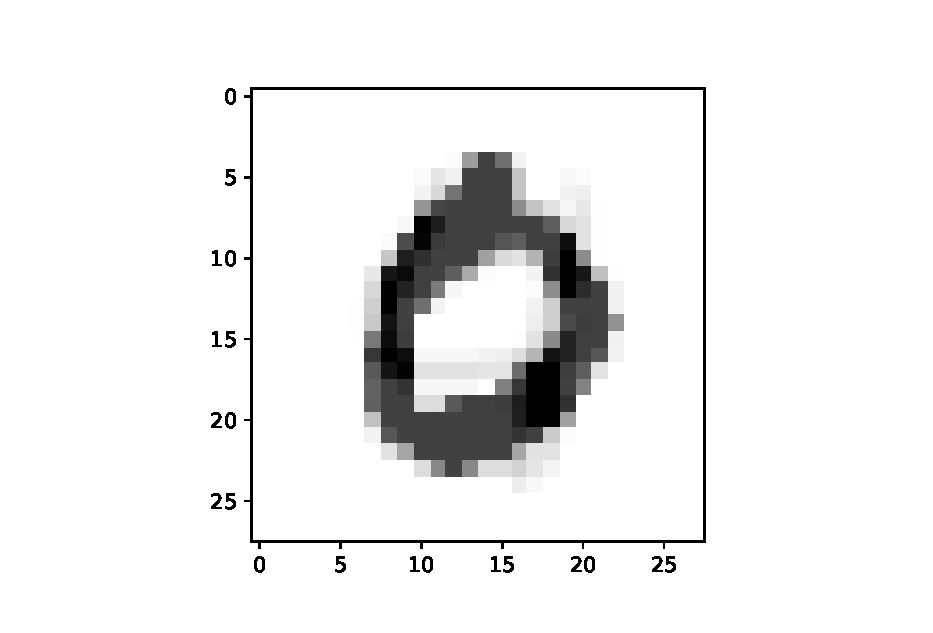
\includegraphics[width=.16\textwidth]{x8.eps}
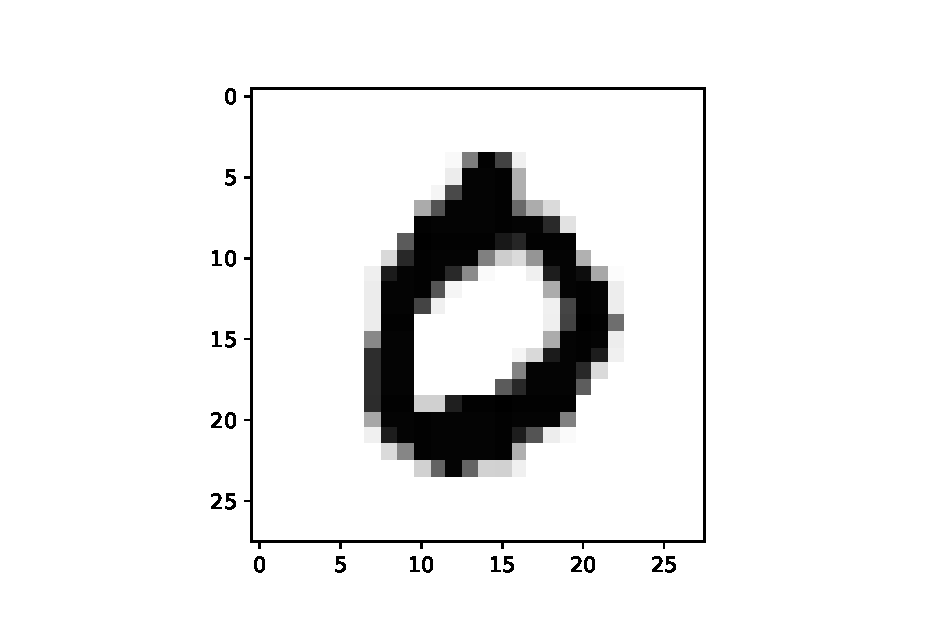
\includegraphics[width=.16\textwidth]{x10.eps} 


 On the other hand, in the original space linear interpolation between two images means the outcome will slowly change from one image to another. It has a smooth fade in fade out effect.
}

\end{homeworkProblem}
\clearpage

%----------------------------------------------------------------------------------------
\begin{homeworkProblem}[The Implementation]
In the implementation section you give a concise insight to the practical aspects of this coding exercise. It mainly mentions the optimization methods used to solve the model equations. Did you encounter numerical or efficiency problems? If yes, how did you solve them?
Provide the link to your git branch of this coding exercise.\newline
Hard limit: One page

\vspace{10pt}
\problemAnswer{ % Answer
Find solution to equation (\ref{error_x}):\\
As stated in exercises sheet, the matrix $\mathbf{W}$ can be found as
\begin{equation}
w_{ij}=\frac{\sum_kC_{jk}^{(i)-1}}{\sum_{lk}C_{lk}^{(i)-1}},
\end{equation}
where $C_{jk}^{(i)}=(\mathbf{x}_i-\mathbf{x}_j)^\top(\mathbf{x}_i-\mathbf{x}_k)$.
\\
\\
Find solution to equation (\ref{error_y}):\\
The optimization problem defined in equation (\ref{error_y}) is equivalent to find $\mathbf{u}_k=(y_{1k},..,y_{Nk})$ for $k=1,..,d$ such that they satisfy
\begin{equation}
\sum_i\mathbf{u}_{ki}=0
\end{equation}
\begin{equation}
\mathbf{u}_k^\top\mathbf{u}_l=\delta_{lk}
\end{equation}
and minimize
\begin{equation}
\sum_k\mathbf{u_k}^\top\mathbf{M}\mathbf{u}_k,
\end{equation}
where $\mathbf{M}=(\mathbb{I}-\mathbf{W})^\top(\mathbb{I}-\mathbf{W})$.
And the optimal solution to this problem are eigenvectors of the matrix $\mathbf{M}$ associated with the smallest $d+1$ eigenvalues and discarding the first eigenvector associated with the eigenvalue 0.\\
\\

Efficiency problem:\\
In the original formulation of LLE stated on the exercise sheet, both neighborhood sets $\mathcal{N}(\mathbf{x}_i)$ and $\mathcal{N}(\mathbf{y}_i)$ are the complete data set. If we are facing a large data set, this approach is clearly inappropriate because the most time consuming part of the program deals with inversing matrix $C$. And matrix the number of neighbors determines the size of matrix $C$. Therefore the number of neighbors need to be predefined as a constant number.\\
Another issue is finding n nearest neighbors. If a naive approach is used, like build up the distance matrix between each pair of points, this part of LLE will cost a lot of time. In my implementation I have used ckdtree as suggested by someone on github. And it is very efficient.\\

Code: LLE is implemented based on the equations in the exercise sheet. \\
\hmwkGitBranch
}
\end{homeworkProblem}
\clearpage

%----------------------------------------------------------------------------------------
% \begin{homeworkProblem}[Your Page]
% Your page gives you space to include ideas, observations and results which do not fall into the categories provided by us. You can also use it as an appendix to include things which did not have space in the other sections.\newline
% No page limit.

% \vspace{10pt}
% \problemAnswer{ % Answer
% Your Answer


% \hmwkGitBranch % defined in line 5
% }
% \end{homeworkProblem}
% \clearpage

\end{document}

